\documentclass[10pt]{beamer}

\usepackage[english]{babel}
\usepackage[utf8]{inputenc}

\usepackage{caption}


\usepackage{listings}
\usepackage{xcolor}
\usepackage{hyperref}
\usepackage{multimedia}

\lstset{
    language=Python,
    basicstyle=\ttfamily\scriptsize, % Size of the font
    keywordstyle=\color{blue}\bfseries,
    stringstyle=\color{red!70!black},
    commentstyle=\color{green!60!black},
    showstringspaces=false,
    frame=single, % Adds a box around the code
    rulecolor=\color{gray!40},
    backgroundcolor=\color{gray!5},
    breaklines=true
}

\usetheme{default}

\definecolor{myred}{RGB}{155, 17, 21}
\definecolor{darkblue}{RGB}{0, 32, 96}
\setbeamercolor{item}{fg=myred}
\setbeamercolor{section in toc}{fg=black}
\setbeamercolor{section in toc shaded}{fg=black}
\setbeamertemplate{footline}[frame number]

% Add this to your preamble
\setbeamercolor{section in toc}{fg=darkblue}
\setbeamertemplate{section in toc}[sections numbered]

\begin{document}

% --- Title Slide ---
{\usebackgroundtemplate{
\includegraphics[width=\paperwidth]{pictures/Dieti}}
\begin{frame}[plain] % 'plain' removes head/footlines for more space
\begin{center}
    \vspace*{0.6cm} % Pulls the header up into the margin space
    {\scriptsize{\Large\textcolor{myred}{D}}IPARTIMENTO DI {\Large\textcolor{myred}{I}}NGEGNERIA {\Large\textcolor{myred}{E}}LETTRICA E {\Large\textcolor{myred}{T}}ECNOLOGIE DELL’{\Large\textcolor{myred}{I}}NFORMAZIONE}
    
    \vspace{0.1cm}
    {\scriptsize SCUOLA POLITECNICA E DELLE SCIENZE DI BASE}
    
    \vfill 
    
    \textbf{LAUREA IN INGEGNERIA DELL'AUTOMAZIONE}
    
    \vspace{0.4cm}
    {\Large\textcolor{myred}{\textbf{Hierarchical VLMs Planning and Control with Ambiguity resolution}}}
    
    \vfill
    
    \begin{columns}[t]
        \begin{column}{0.45\textwidth}
            \begin{flushleft} \small
                Candidato:\\
                \textbf{Vincenzo Palomba}\\
            \end{flushleft}
        \end{column}
        \begin{column}{0.45\textwidth}
            \begin{flushright} \small
                Relatori:\\
                \textbf{Prof. Alberto Finzi} \\
            \end{flushright}
        \end{column}
    \end{columns}
    
    \vspace{0.4cm}
    {\footnotesize Academic Year 2025/2026}
\end{center}
\end{frame}
}


% --- Table of Contents ---
\begin{frame}
\frametitle{Outline} 
        \vspace{0.2cm}
        \tableofcontents[hideallsubsections]
        \vspace{0.2cm}
\end{frame}

% --- What to write ---
% Planning Layer: Introduction to planning: from classical to ai-planning. VLM: what is, principal architectures, what i've used. Ambiguity resolution. VLM to PDDL pipeline: schema and description.
% Executive Layer: introduction. BTs intro. My implementation
% Control Layer: rrt motion planner. rl and il

\section{Planning Layer}
\begin{frame}
    \frametitle{Neuro-Symbolic Planning architecture}
     
\end{frame}

\begin{frame}
\frametitle{VLM Architectures}
\begin{columns}[T] % [T] aligns columns at the top
    % https://www.ibm.com/think/topics/vision-language-models?utm_medium=OSocial&utm_source=Youtube&utm_content=WAIWW&utm_id=YT-101-What-are-vision-language-models-(VLMs)
    % --- Left Column: VLM Schema Image ---
    \begin{column}{0.48\textwidth}
        \begin{figure}
            \centering
            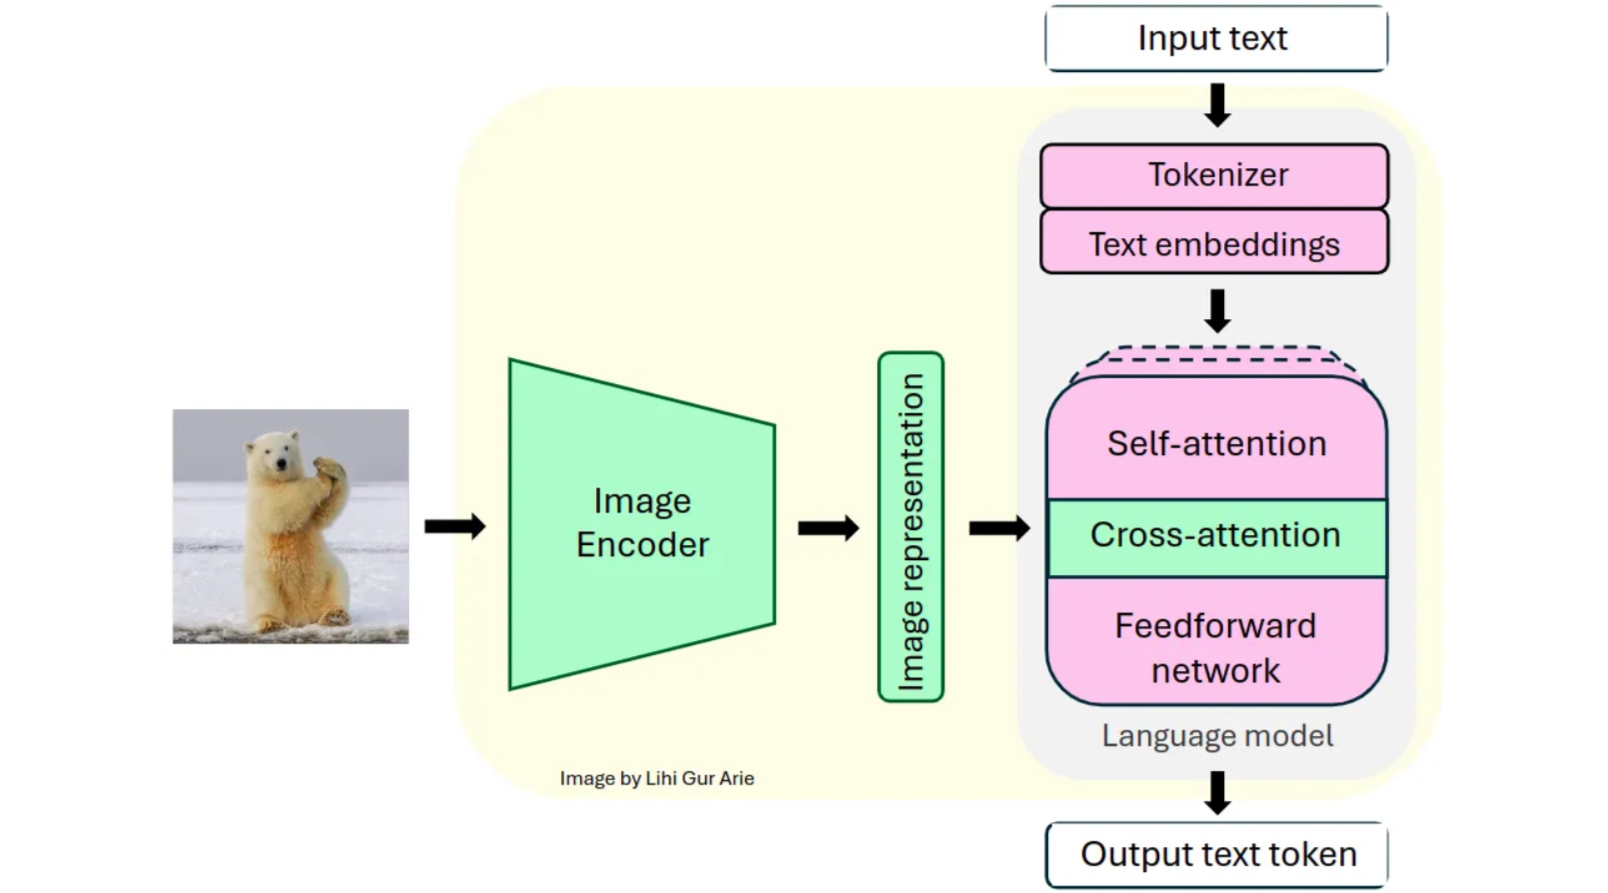
\includegraphics[width=\linewidth]{pictures/llama3.png}
            \caption{llama3 VLM architecture}
        \end{figure}

        \vspace{0.2cm}
        {\centering \fbox{\scriptsize Image + Text $\longrightarrow$ VLM $\longrightarrow$ Text Output} \par}
    \end{column}

    % --- Right Column: Text Boxes ---
    \begin{column}{0.48\textwidth}
        
        \setbeamercolor{verdictbox}{bg=darkblue,fg=white}
        \begin{beamercolorbox}[sep=4pt,shadow=true,rounded=true]{verdictbox}
            \usebeamerfont{title} \small \textbf{Language Encoder (Transformer)} \\ 
            \vspace{0.05cm} 
            \tiny % Using tiny to fit two boxes vertically on the right
            \begin{itemize}
                \setlength\itemsep{0em}
                \item Encoders transform sequences into numerical representation called \textbf{embeddings}.
                \item A \textbf{self-attention mechanism} allows focus on important tokens.
                \item \textbf{Decoders} output the most statistically probable output.
            \end{itemize}
        \end{beamercolorbox}
        
        \vspace{0.3cm} % Spacing between the two text boxes
        
        \setbeamercolor{verdictbox}{bg=darkblue,fg=white}
        \begin{beamercolorbox}[sep=4pt,shadow=true,rounded=true]{verdictbox}
            \usebeamerfont{title} \small \textbf{Vision Encoder (CNN / ViT)} \\
            \vspace{0.05cm}
            \tiny % Using tiny to fit two boxes vertically on the right
            \begin{itemize}
                \setlength\itemsep{0em}
                \item Typically utilizes Convolutional Neural Networks (CNNs) or Visual Transformers (ViTs).
                \item A ViT processes an image into patches and treats them as sequences, akin to tokens.
            \end{itemize}
        \end{beamercolorbox}
    \end{column}
    
\end{columns}
\end{frame}

\begin{frame}
    \frametitle{VLM Training methodologies}
    It is the mechanism that allow fusing information from both vision and language encoders so to correlate images with text and make decision on the 2 modalities togheter:
    \begin{itemize}
        \item Contrasive learning: uses joint or shared embedding space. The VLM is trained on datasets of image-text pairs and learns to minimize the distance between embeddings of matching pairs and maximize it for nonmatching pairs.
        \item Masking: models learn to predict randomly obscured parts of an input text or image.
        \item Generative model training: entails learning to generate new data
        \item Pretrained models: A pretrained LLM and a pretrained vision encoder can be used, with an added mapping network layer that aligns or projects the visual representation of an image to the LLM’s input space.
    \end{itemize}
\end{frame}

\begin{frame}
\frametitle{Qwen 2.5-VL}
\begin{columns}[T] % [T] aligns columns at the top
    % https://towardsai.com/p/machine-learning/qwen2-5-vl-a-hands-on-code-walkthrough
    \begin{column}{0.5\textwidth}
        \textbf{VLM Architecture}
        \begin{itemize}
            \item Qwen2.5 LM Decoder
            \item ViT:3D convolution to split input visual data into a series of 14*14 patches
            \item process video info: preprocessor for dynamic image size adjustment, dynamic frame extraction
        \end{itemize}
        \vspace{0.4cm}
    \end{column}

    \begin{column}{0.5\textwidth}
        \begin{figure}
            \centering
            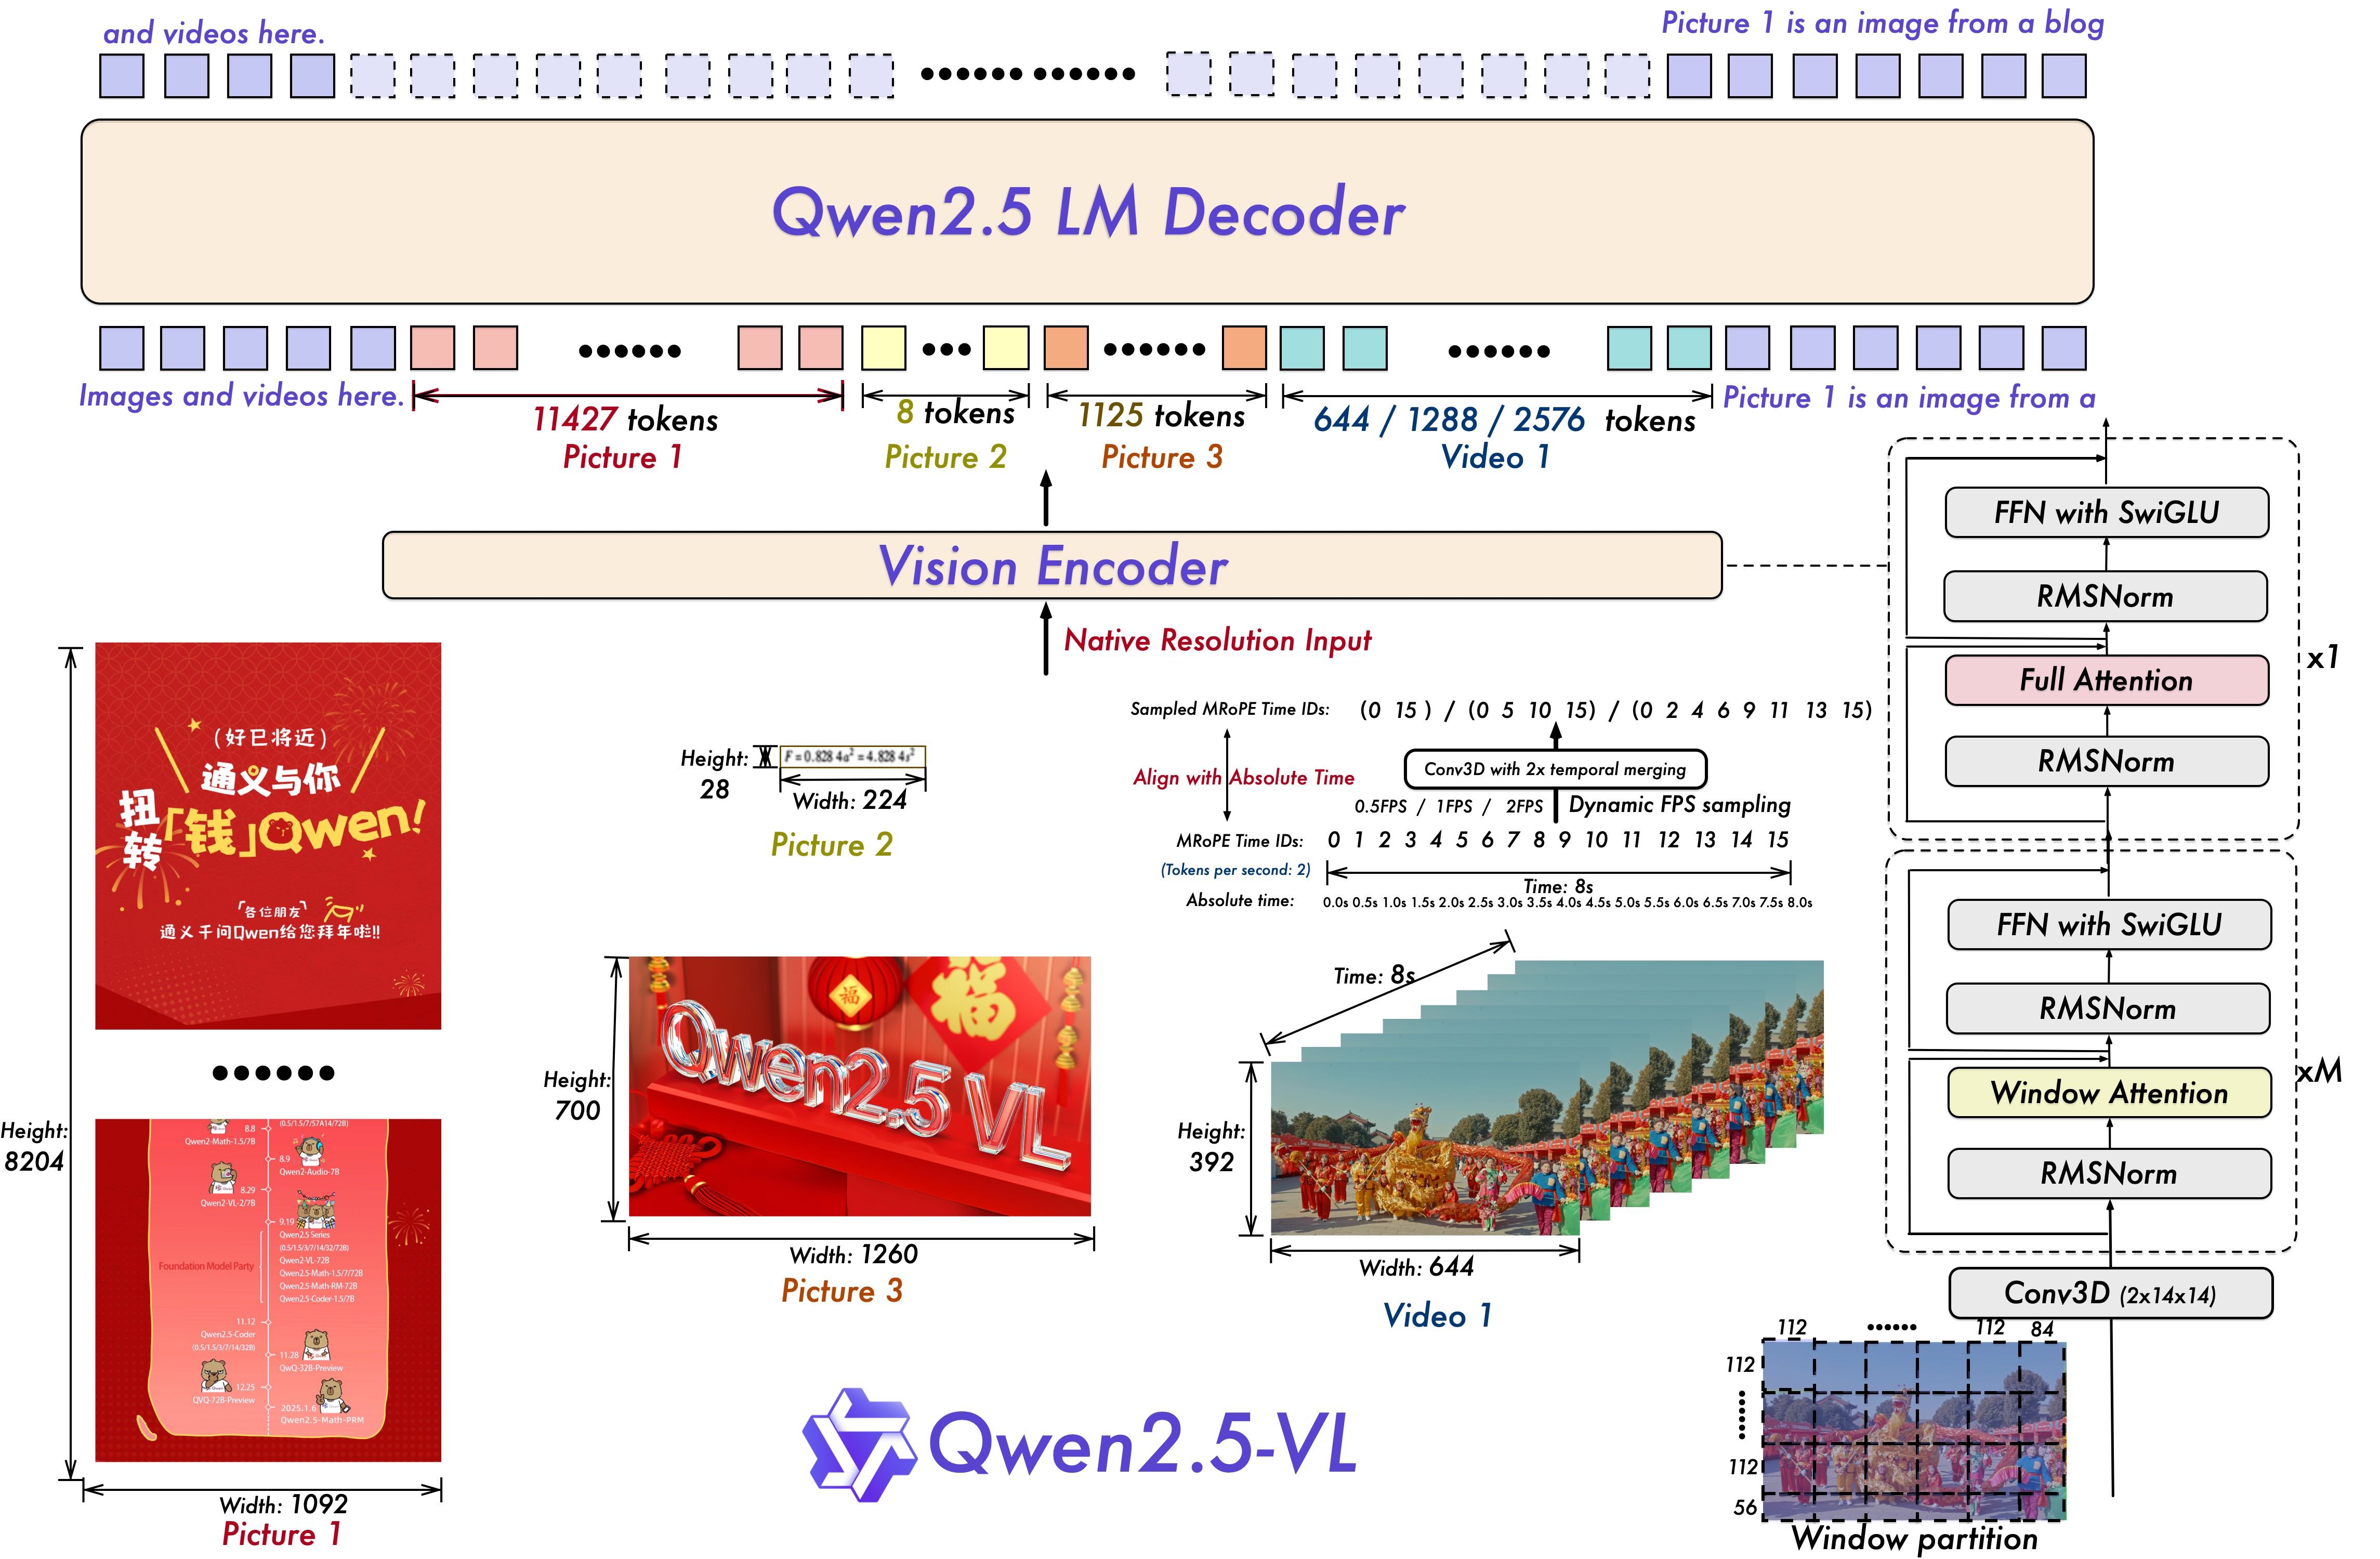
\includegraphics[width=\textwidth]{pictures/qwen2.5vl_arc.jpeg}
        \end{figure}
    \end{column}
\end{columns}


\vspace{0.2cm}
\setbeamercolor{verdictbox}{bg=darkblue,fg=white}
\begin{beamercolorbox}[sep=8pt,center,shadow=true,rounded=true]{verdictbox}
    \usebeamerfont{title} \small \textbf{Why this choice?} \\ 
    \scriptsize 
\end{beamercolorbox}

\end{frame}

\begin{frame}
    \frametitle{Ambiguity resolution}


\end{frame}

\begin{frame}
    \frametitle{PDDL planning}
    
\end{frame}

\begin{frame}
    \frametitle{PDDL problem generation experiments}
\end{frame}

\section{Executive Layer}


\section{Control Layer}

\section{Setup and Experimental Results}

\section{Conclusion}

\end{document}